\chapter{Proposed Methodology and System Design}
\label{ch:method}

\section{Introduction}

This chapter describes the design and implementation of the Q\&A based interactive storytelling system developed in this dissertation. It starts with the feasibility study and the project plan, then gives an overview of the system and the research workflow. It then explains each part in turn: the question framework, the way answers are turned into a story context and a prompt, the five-phase story model, the seven backend modules, the multimodal pipelines and the reader analytics. The implementation, the hardware and software used, and the evaluation method are described at the end of the chapter.

\section{Feasibility Study}
\label{sec:feasibility}

\subsection{Technical Feasibility}

Every part of the system can be built with mature and freely available technology. LLM inference is possible on an ordinary laptop through Ollama~\citep{ollama2024} (16\,GB RAM and no dedicated GPU for 7B-class models) and in the cloud through the free Groq tier, which allows 14,400 requests per day. Text-to-image synthesis is available without an API key through Pollinations.ai~\citep{pollinations2024api}. Voice synthesis is built into all major browsers through the Web Speech API~\citep{w3c2024webspeech}, and ambient music can be streamed from the SoundHelix CDN~\citep{brichta2024soundhelix}. The backend can be written in Python with FastAPI~\citep{ramirez2024fastapi}, SQLite and Pydantic~\citep{colvin2024pydantic}, and the frontend in plain HTML, CSS and JavaScript with D3.js~\citep{bostock2011d3} for charts.

\subsection{Economic Feasibility}

The system can be developed and run at almost no cost. Development used Ollama and the free Groq tier; images are generated free of charge through Pollinations; and audio streaming uses very little bandwidth from a public CDN. The recurring cost during the user study, with 15 participants over two weeks, was zero. All development was done on one laptop, so no external funding was required.

\subsection{Operational Feasibility}

The Q\&A protocol follows the way a human author collects a brief from a client, through a short interview about setting, characters, theme and plot, so it is familiar to users. The question budget (4 to 17 questions) lets each user choose how much effort to spend. All steps take place on a single page, and the settings and admin panels expose every option without any change to code.

\subsection{Legal and Ethical Feasibility}

All third-party services used (Pollinations, SoundHelix, Groq, Hugging Face and OpenAI) allow non-commercial research use, and SoundHelix explicitly allows direct linking. No personally identifiable data is stored permanently: session data is kept in memory and in a local SQLite file. The user study was carried out with informed consent.

\section{Project Planning and Scheduling}
\label{sec:schedule}

The project ran from August 2025 to May 2026. The work was broken down into eleven activities in five phases:

\begin{enumerate}
    \item \textbf{Planning and design} (weeks 1--12): literature survey, requirement analysis with the guide, and system design covering the architecture, module boundaries, data flow, REST interface and database schema.
    \item \textbf{Implementation} (weeks 10--23): the seven backend modules, the LLM provider layer with Ollama, Groq, Hugging Face and OpenAI clients, and the frontend with the landing page, question form, story view, admin panel and settings panel.
    \item \textbf{Multimodal features} (weeks 20--26): the image pipeline with the prompt extractor and request queue, TTS narration, ambient music, and the Story Map and Character Graph.
    \item \textbf{Evaluation} (weeks 25--29): automatic generation of 50 stories, the user study with 15 participants, and the consistency-checker evaluation.
    \item \textbf{Documentation} (weeks 28--36): the dissertation report, a research paper, and the final review and presentation.
\end{enumerate}

The timeline is shown in Figure~\ref{fig:gantt}. Some activities overlap on purpose; for example, frontend work ran alongside backend work, and multimodal integration overlapped with the end of frontend development.

\begin{figure}[H]
    \centering
    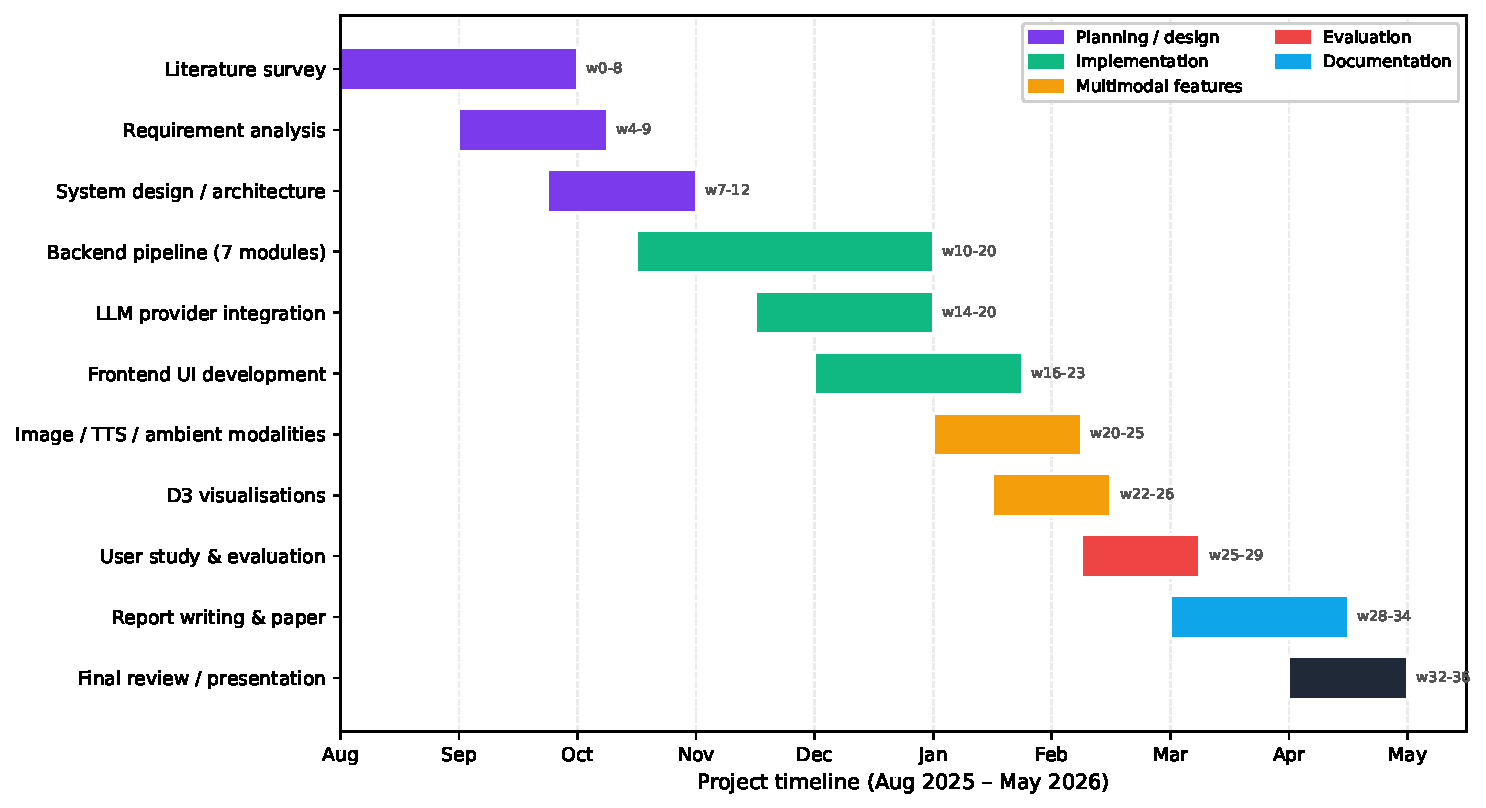
\includegraphics[width=\textwidth]{images/gantt.pdf}
    \caption{Project Gantt chart (August 2025 to May 2026).}
    \label{fig:gantt}
\end{figure}

The main risks identified during planning and the way each was handled are listed in Table~\ref{tab:risks}.

\begin{table}[H]
\centering
\caption{Risk register and mitigation.}
\label{tab:risks}
\renewcommand{\arraystretch}{1.2}
\small
\begin{tabular}{|p{4.0cm}|p{3.2cm}|p{6.0cm}|}
\hline
\textbf{Risk} & \textbf{Likelihood / Impact} & \textbf{Mitigation} \\
\hline
Rate limits of the free image API & High / High     & Serial request queue with 1.2\,s spacing and a 35\,s watchdog \\
LLM provider downtime             & Medium / Medium & Provider-independent layer that can be switched through \texttt{/api/settings} \\
Loss of narrative coherence       & Medium / High   & Sliding-window context and a consistency checker \\
Browser blocks audio autoplay     & High / Low      & Start audio only after a real user click \\
Delay in the user study           & Medium / Medium & Rolling sessions over two weeks, remote participation allowed \\
Cross-origin errors for CDN audio & Medium / Low    & Plain \texttt{HTMLAudio} without the \texttt{crossOrigin} attribute \\
\hline
\end{tabular}
\end{table}

\section{System Overview}

The system is organised in layers, shown in Figure~\ref{fig:arch}. The \emph{presentation layer} is a single-page web application that shows the questions, the story, the images and the analytics, and plays narration and music. The \emph{application layer} is a FastAPI server that exposes the REST endpoints and manages sessions. The \emph{modular core} contains the seven backend modules that turn answers into a story. At the bottom, a pluggable \emph{LLM provider layer} connects the core to Ollama, Groq, Hugging Face or OpenAI. Each layer depends only on the layer below it, so a provider can be changed or a module improved without touching the rest.

\begin{figure}[H]
    \centering
    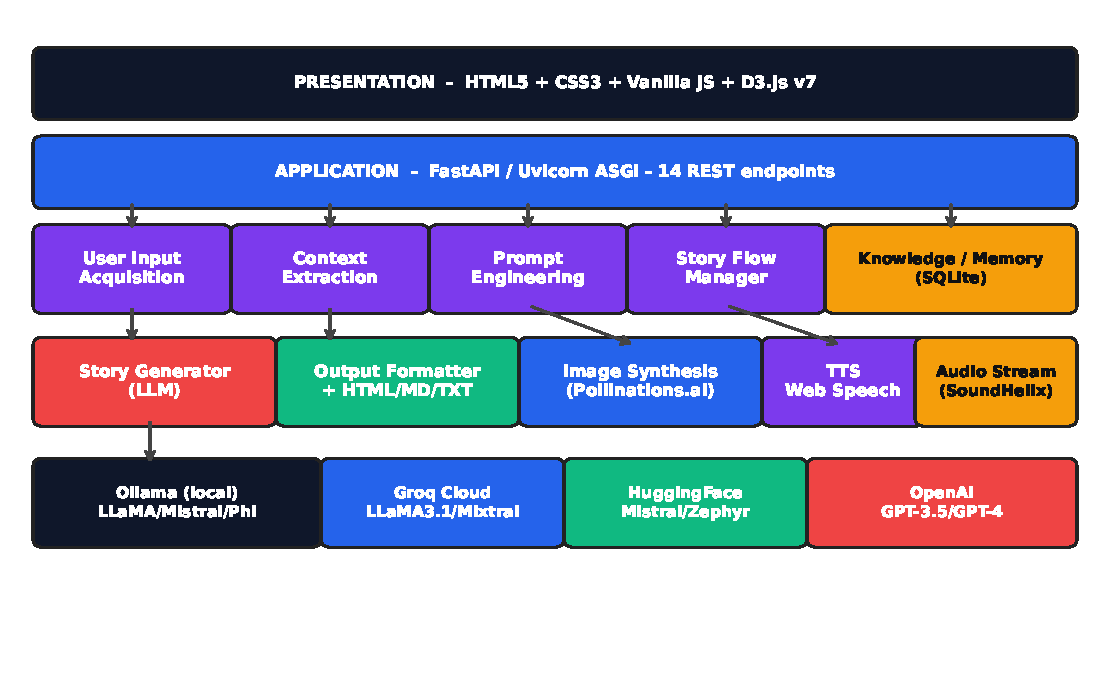
\includegraphics[width=\textwidth]{images/f07_arch.pdf}
    \caption{Layered architecture of the proposed system.}
    \label{fig:arch}
\end{figure}

\section{Research Design}

The research followed the workflow shown in Figure~\ref{fig:workflow}. Requirements were gathered from the literature and from discussion with the guide, the system was designed and built module by module, and the multimodal features were added on top of a working text pipeline. The complete system was then tested and evaluated with automatic measurements and a user study. Problems found in testing were fixed and the affected tests were run again.

\begin{figure}[H]
\centering
\begin{tikzpicture}[
    node distance=5mm,
    box/.style={draw, thick, rounded corners, fill=blue!8, minimum width=7cm, minimum height=8mm, align=center, font=\small},
    term/.style={draw, thick, ellipse, fill=green!15, minimum width=3cm, font=\small\bfseries},
    dec/.style={draw, thick, diamond, aspect=2.6, fill=orange!15, font=\small, inner sep=1pt, align=center},
    arr/.style={-{Stealth[length=2mm]}, thick}
]
\node[term] (start) {Start};
\node[box, below=of start] (a) {Literature survey and requirement analysis};
\node[box, below=of a] (b) {Design architecture, modules, API and schema};
\node[box, below=of b] (c) {Implement Q\&A, context, prompt and LLM modules};
\node[box, below=of c] (d) {Add story-flow manager and consistency checker};
\node[box, below=of d] (e) {Add images, narration, music and analytics};
\node[box, below=of e] (f) {Unit, integration, API and UI testing};
\node[dec, below=of f] (g) {All tests\\pass?};
\node[box, below=8mm of g] (h) {Evaluate: 50 stories and user study ($n=15$)};
\node[box, below=of h] (i) {Analyse results and write report};
\node[term, below=of i] (stop) {End};
\draw[arr] (start) -- (a);
\foreach \x/\y in {a/b, b/c, c/d, d/e, e/f, f/g, h/i, i/stop} \draw[arr] (\x) -- (\y);
\draw[arr] (g) -- node[right, font=\footnotesize] {Yes} (h);
\draw[arr] (g.east) -- ++(1.9,0) |- node[pos=0.25, right, font=\footnotesize] {No (fix)} (c.east);
\end{tikzpicture}
\caption{Research workflow followed in this dissertation.}
\label{fig:workflow}
\end{figure}

\section{Question-and-Answer Framework}
\label{sec:qa}

\subsection{Question Pool}

The elicitation protocol has seventeen questions divided among four narrative phases, as shown in Figure~\ref{fig:qa}:

\begin{itemize}
    \item \textbf{Setting}: the kind of world, the time period and the atmosphere of the story.
    \item \textbf{Character}: the protagonist's name, personality and goal, the antagonist, and supporting characters.
    \item \textbf{Theme}: the genre, the tone and the central message.
    \item \textbf{Plot}: the type of conflict, the plot style, the pacing and the kind of ending.
\end{itemize}

\begin{figure}[H]
    \centering
    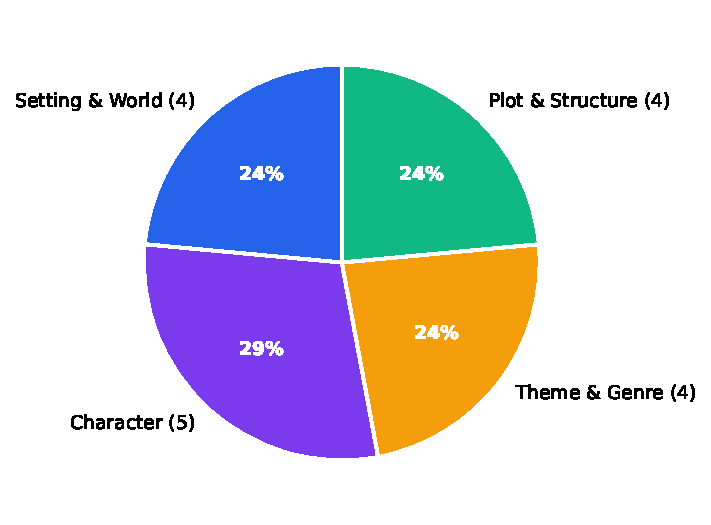
\includegraphics[width=0.65\textwidth]{images/f08_qa.pdf}
    \caption{Distribution of the 17 questions across the four phases.}
    \label{fig:qa}
\end{figure}

The user selects a budget of 4 (Quick), 8 (Balanced), 12 (Detailed) or 17 (Full) questions. The system always presents the first $N$ questions in phase order, so even the smallest budget touches all four dimensions. Every question offers multiple-choice options and a ``Write my own'' option for a free-text answer. In addition, the user may add entirely new questions with their own answers.

\subsection{Elicitation Protocol}

Let $\mathcal{Q}=\{q_1,\ldots,q_{17}\}$ be the ordered question pool. The user selects a budget $N\in\{4,8,12,17\}$ and gives an answer $a_i$ to each question $q_i$ with $i \le N$. The user may also add $M$ new question-answer pairs $(\tilde q_j, \tilde a_j)$, which receive the identifiers $\mathrm{custom\_q\_}j$. The complete response set is
\begin{equation}
R = \{(q_i, a_i)\}_{i=1}^{N} \;\cup\; \{(\mathrm{custom\_q\_}j,\ \tilde a_j)\}_{j=1}^{M},
\end{equation}
and it is sent to the context-extraction module as a JSON dictionary.

\subsection{Context Projection and Prompt Construction}

For each pair $(q_i,a_i)$ the context-extraction module applies a fixed projection $\pi_i$ that writes the answer into a typed field of a \texttt{StoryContext} object, for example \texttt{setting\_type}, \texttt{antagonist} or \texttt{plot\_style}. Answers whose identifiers are not known to the system, including all user-added questions, are stored word for word in a dictionary $D$ called \texttt{custom\_elements}. The final prompt $P$ is built as
\begin{equation}
P = T(\mathbf{c}) \oplus \sigma(D),
\end{equation}
where $T$ is the prompt template for the current story phase, $\mathbf{c}$ is the structured context, $\sigma$ turns the dictionary $D$ into a list of natural-language bullet points, and $\oplus$ joins the two strings. This design means that a new question added by the user reaches the model without any change to code or to the database schema. Figure~\ref{fig:customq} shows this routing.

\begin{figure}[H]
    \centering
    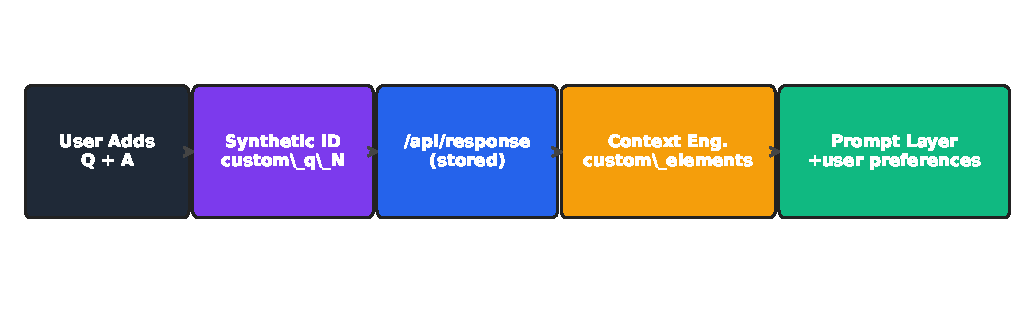
\includegraphics[width=0.95\textwidth]{images/f16_customq.pdf}
    \caption{Routing of user-added questions from the interface to the LLM prompt.}
    \label{fig:customq}
\end{figure}

\section{Five-Phase Story Progression}
\label{sec:phases}

The story-flow manager is a finite-state machine based on Freytag's pyramid~\citep{freytag1900drama}. The story moves through five phases according to its total word count, as listed in Table~\ref{tab:phases}. The current phase selects the prompt template: the introduction template asks the model to set the scene and introduce the characters, the climax template asks for the main confrontation, and the resolution template asks the model to close open plot threads. Figure~\ref{fig:phases} shows the observed word counts per phase; the rising action takes the largest share of the text (about 820 words), which agrees with narrative theory.

\begin{table}[H]
\centering
\caption{Word-count thresholds of the five story phases.}
\label{tab:phases}
\renewcommand{\arraystretch}{1.2}
\begin{tabular}{|l|c|l|}
\hline
\textbf{Phase} & \textbf{Word range} & \textbf{Purpose of the prompt} \\
\hline
Introduction   & 0--400       & Establish setting and characters \\
Rising action  & 400--1200    & Develop conflict and complications \\
Climax         & 1200--1800   & Main confrontation or turning point \\
Falling action & 1800--2400   & Consequences of the climax \\
Resolution     & $>$ 2400     & Resolve open threads and conclude \\
\hline
\end{tabular}
\end{table}

\begin{figure}[H]
    \centering
    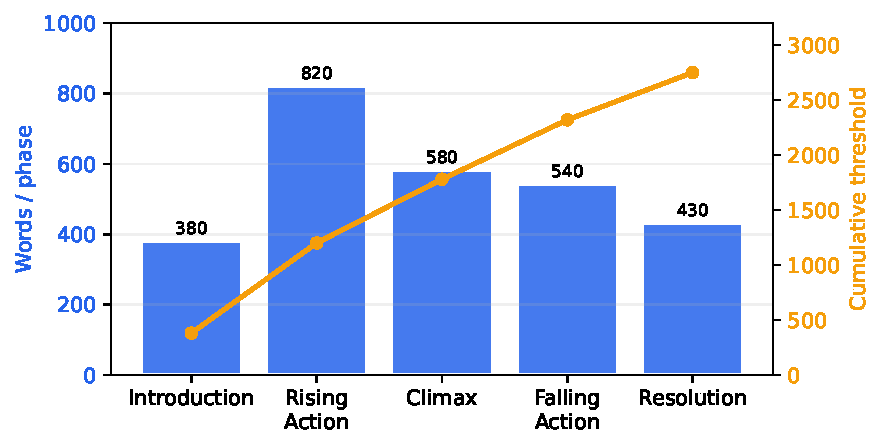
\includegraphics[width=0.9\textwidth]{images/f04_phases.pdf}
    \caption{Word-count distribution across the five story phases.}
    \label{fig:phases}
\end{figure}

\section{Generation Loop}

Each turn of the story follows Algorithm~\ref{alg:loop}. The model sees the structured context and only the last $k$ segments of the story, which keeps the prompt within the context window while preserving the most recent events. Image generation starts in parallel with post-processing so that the picture is often ready when the user finishes reading.

\begin{algorithm}[H]
\caption{Story generation loop for one turn}
\label{alg:loop}
\begin{algorithmic}[1]
\Require session $s$, structured context $\mathbf{c}$, custom elements $D$, user choice $u$ (empty on the first turn)
\Ensure formatted segment and choices for the next turn
\State $H \gets$ last $k$ segments of session $s$ \Comment{sliding window, $k=4$}
\State $\phi \gets$ current phase from total word count
\State $P \gets T_{\phi}(\mathbf{c}, H, u) \oplus \sigma(D)$
\State $y \gets \textsc{LLM}(P)$ \Comment{active provider}
\State $y \gets \textsc{Format}(y)$ \Comment{clean text, style dialogue}
\State update character and plot-thread trackers with $y$
\State run consistency checks on $y$ against $H$ and $\mathbf{c}$
\State start image request for $y$ asynchronously
\State save $y$ to the database; update word count
\State \Return $y$ and generated choices
\end{algorithmic}
\end{algorithm}

\section{Backend Modules}
\label{sec:modules}

The backend has seven modules with clear responsibilities and typed Pydantic interfaces.

\subsection{Module 1: User Input Acquisition}

This module holds the question pool and serves it through two endpoints: \texttt{/api/questions/all} returns all questions grouped by phase, and \texttt{/api/question/next} supports an older one-question-at-a-time mode. Answers are received through \texttt{POST /api/response} and validated. The landing page (Figure~\ref{fig:ui-landing}) lets the user choose a budget, and the question form (Figure~\ref{fig:ui-form}) shows each question with its options and a dashed ``Write my own'' chip.

\begin{figure}[H]
    \centering
    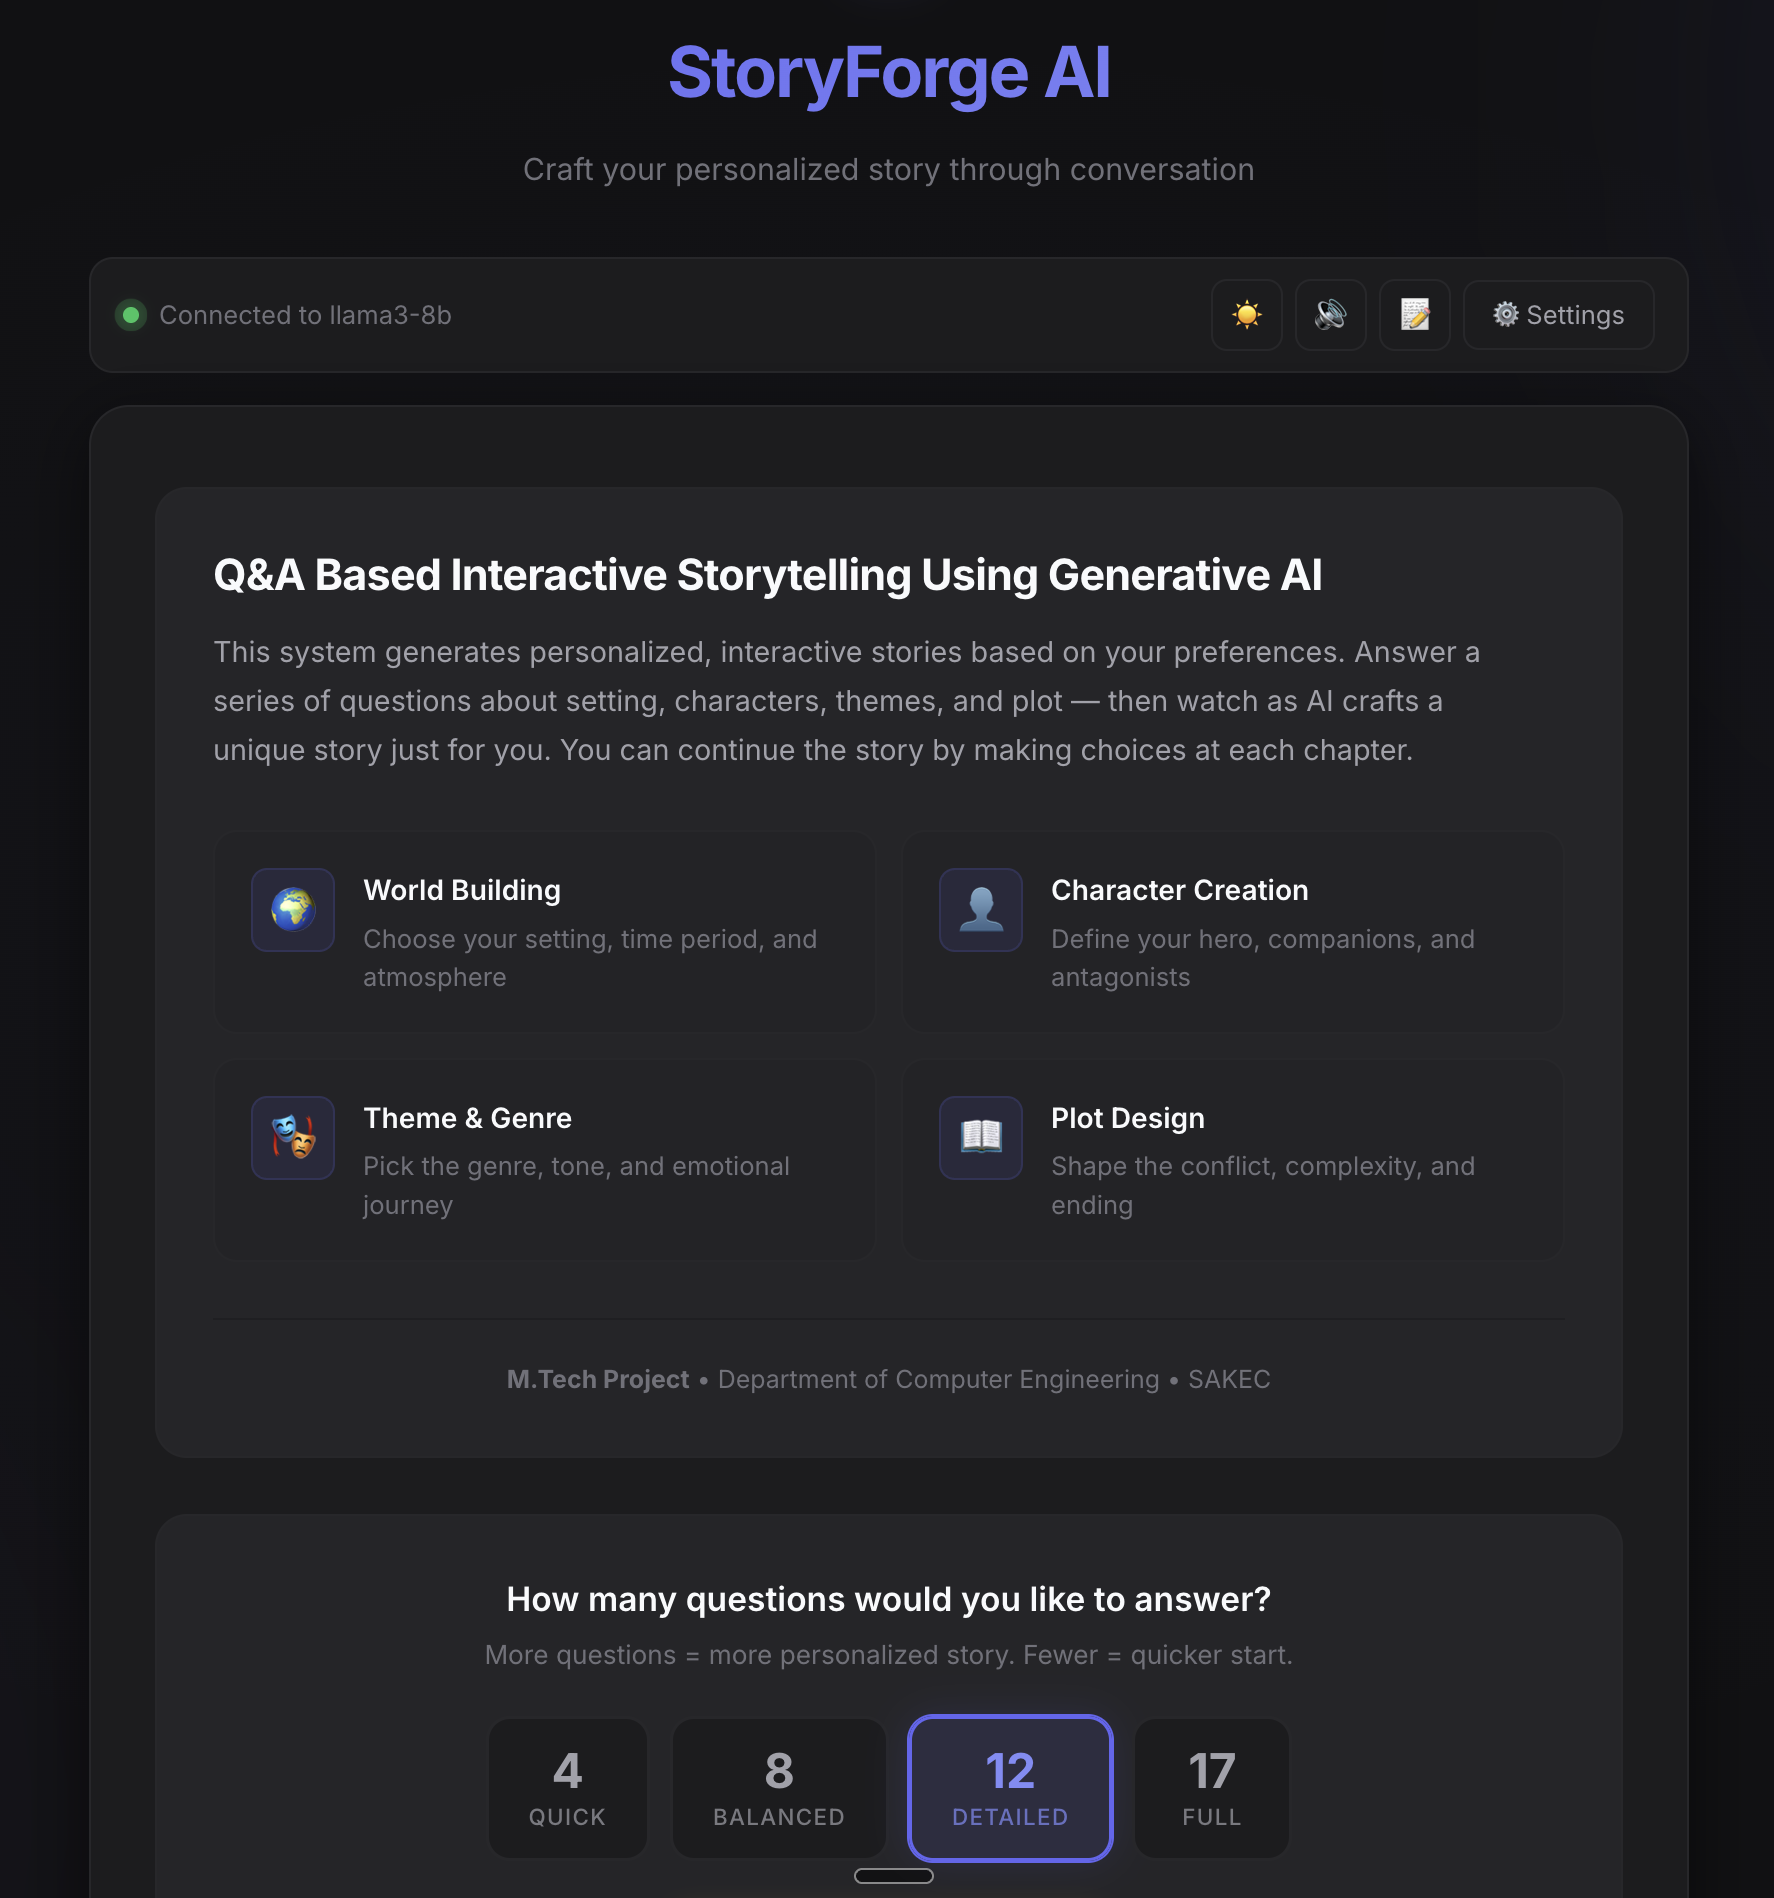
\includegraphics[width=0.85\textwidth]{images/s01_landing.png}
    \caption{Landing page with the choice of question budget.}
    \label{fig:ui-landing}
\end{figure}

\begin{figure}[H]
    \centering
    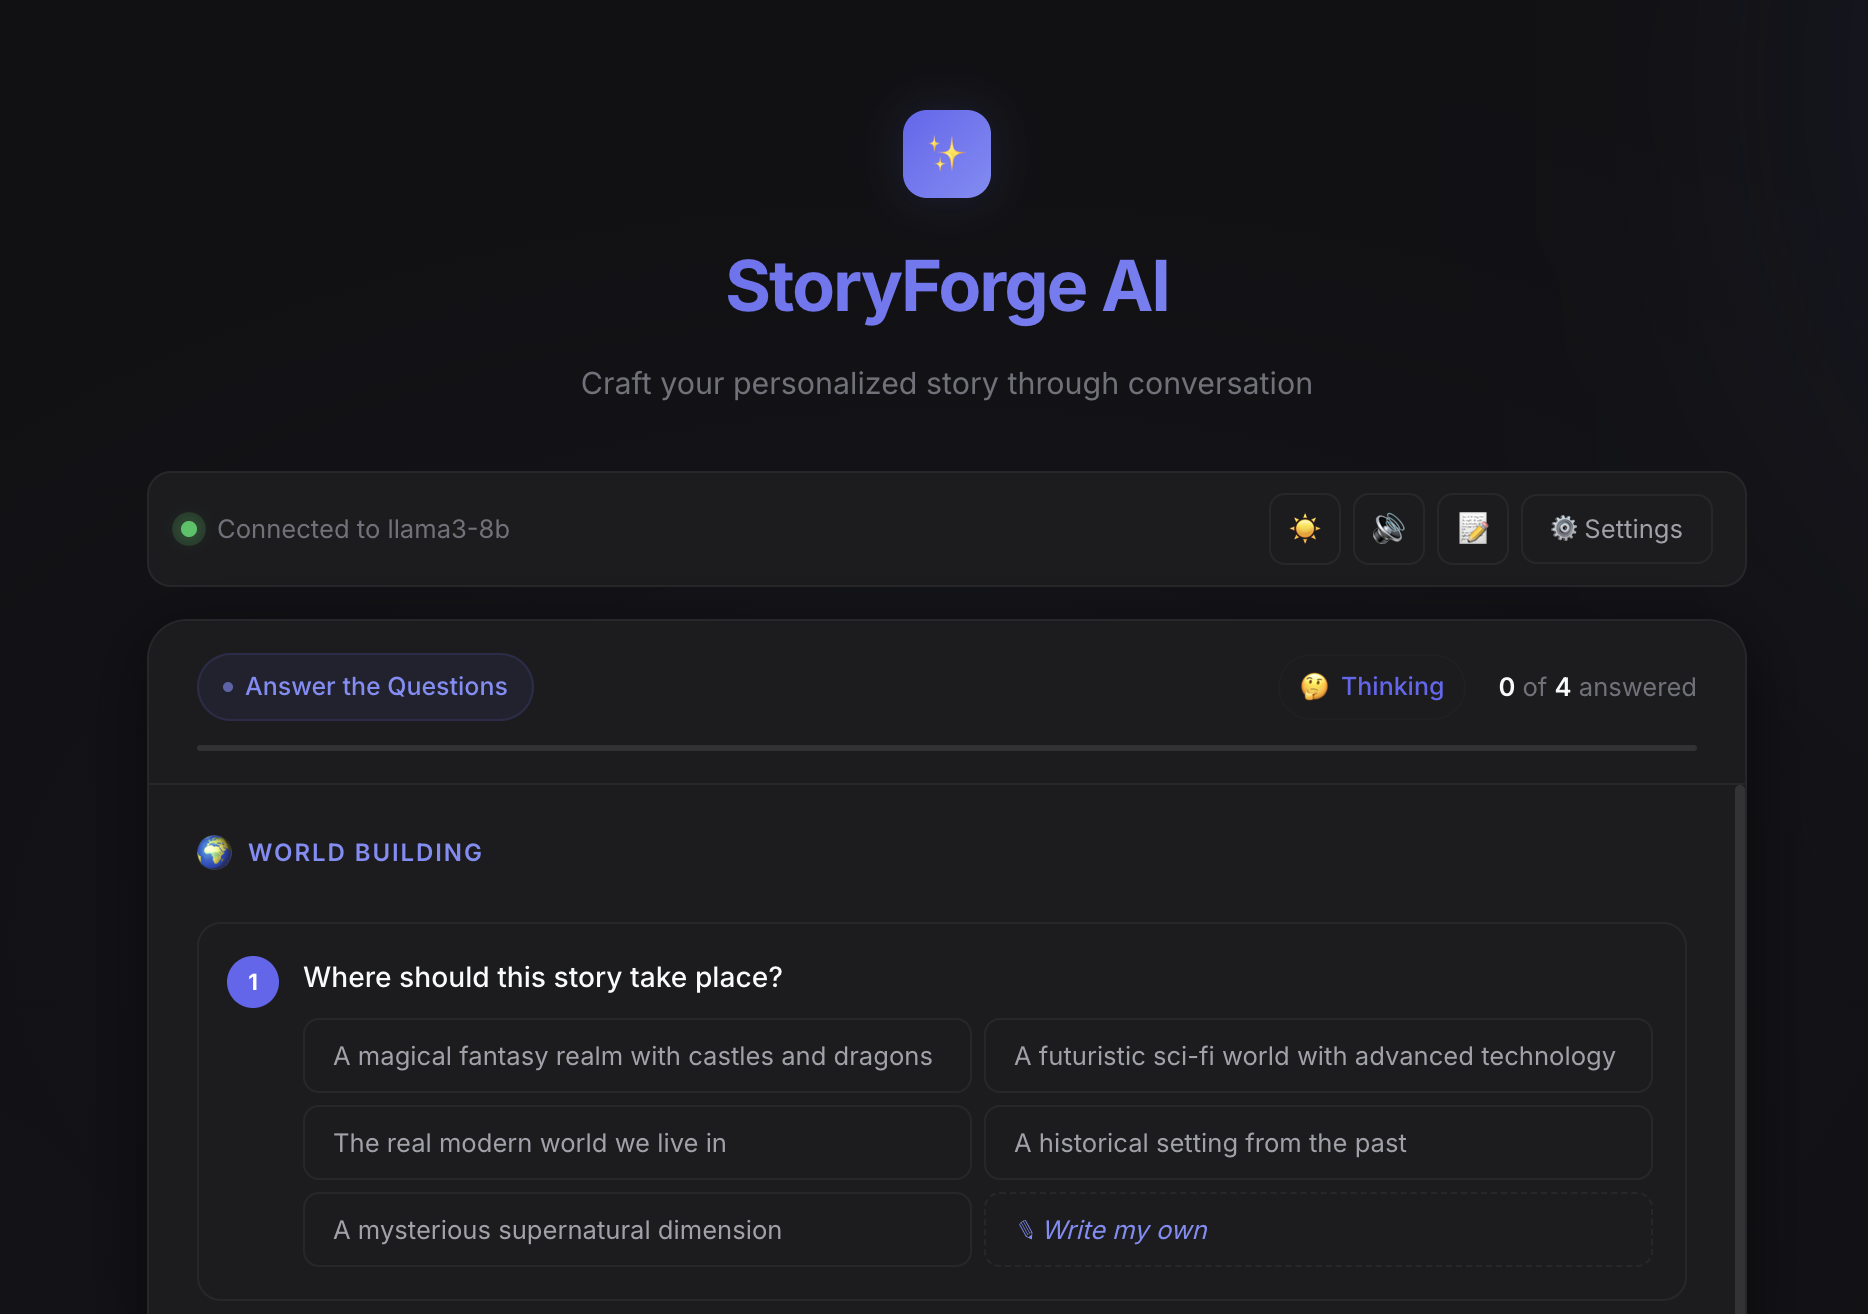
\includegraphics[width=0.85\textwidth]{images/s02_questions.png}
    \caption{Single-page question form with custom-answer option.}
    \label{fig:ui-form}
\end{figure}

\subsection{Module 2: Context Extraction Engine}

This module fills the \texttt{StoryContext} object. It works in two passes: first it classifies answers with keyword dictionaries (six genres, five setting types and five conflict types), and then it extracts proper names with regular expressions. Identifiers that begin with \texttt{custom\_} are routed into \texttt{custom\_elements}:

\begin{lstlisting}[language=Python]
elif question_id.startswith("custom_"):
    self.context.custom_elements[question_id] = answer
\end{lstlisting}

\subsection{Module 3: Knowledge and Memory}

This module stores sessions, answers, segments and preferences in SQLite, keeps an in-memory LRU cache for active sessions, and provides the sliding-window helper used in Algorithm~\ref{alg:loop}:

\begin{lstlisting}[language=Python]
def get_recent_context(session_id: str, k: int = 4) -> str:
    """Return the concatenated text of the last k segments."""
\end{lstlisting}

\subsection{Module 4: Prompt Engineering}

This module holds six prompt families: the system prompt, the initial-segment prompt, the continuation prompt, the climax prompt, the resolution prompt and the choice-generation prompt. Each is filled with fields from \texttt{StoryContext}, and genre-specific guidance is added (for example, magic systems for fantasy, clue placement and red herrings for mystery, and emotional pacing for romance). User-added preferences are appended at the end:

\begin{lstlisting}[language=Python]
if context.custom_elements:
    extras = "\n".join(f"- {v}" for v in context.custom_elements.values() if v)
    if extras:
        prompt += "\n\nAdditional user preferences to honour:\n" + extras
\end{lstlisting}

\subsection{Module 5: Story Generator}

The story generator defines an abstract class \texttt{BaseLLMClient} with four concrete clients, compared in Table~\ref{tab:providers}. A factory creates the client named in the configuration. The settings panel (Figure~\ref{fig:ui-settings}) lets a non-technical user choose the provider, model, temperature and features; a change is sent to \texttt{POST /api/settings}, which replaces the client without restarting the server.

\begin{table}[H]
\centering
\caption{LLM providers supported by the system.}
\label{tab:providers}
\renewcommand{\arraystretch}{1.2}
\begin{tabular}{|l|l|l|c|}
\hline
\textbf{Provider} & \textbf{Models} & \textbf{Cost} & \textbf{Latency} \\
\hline
Ollama       & LLaMA 3.2, Mistral, Phi    & Free (local)        & 8--15\,s \\
Groq         & LLaMA 3.1 8B/70B, Mixtral  & Free, 14,400/day    & 1--3\,s \\
Hugging Face & Mistral-7B, Zephyr, Falcon & Free (rate-limited) & 6--10\,s \\
OpenAI       & GPT-3.5-turbo, GPT-4       & Paid per token      & 2--4\,s \\
\hline
\end{tabular}
\end{table}

\begin{figure}[H]
    \centering
    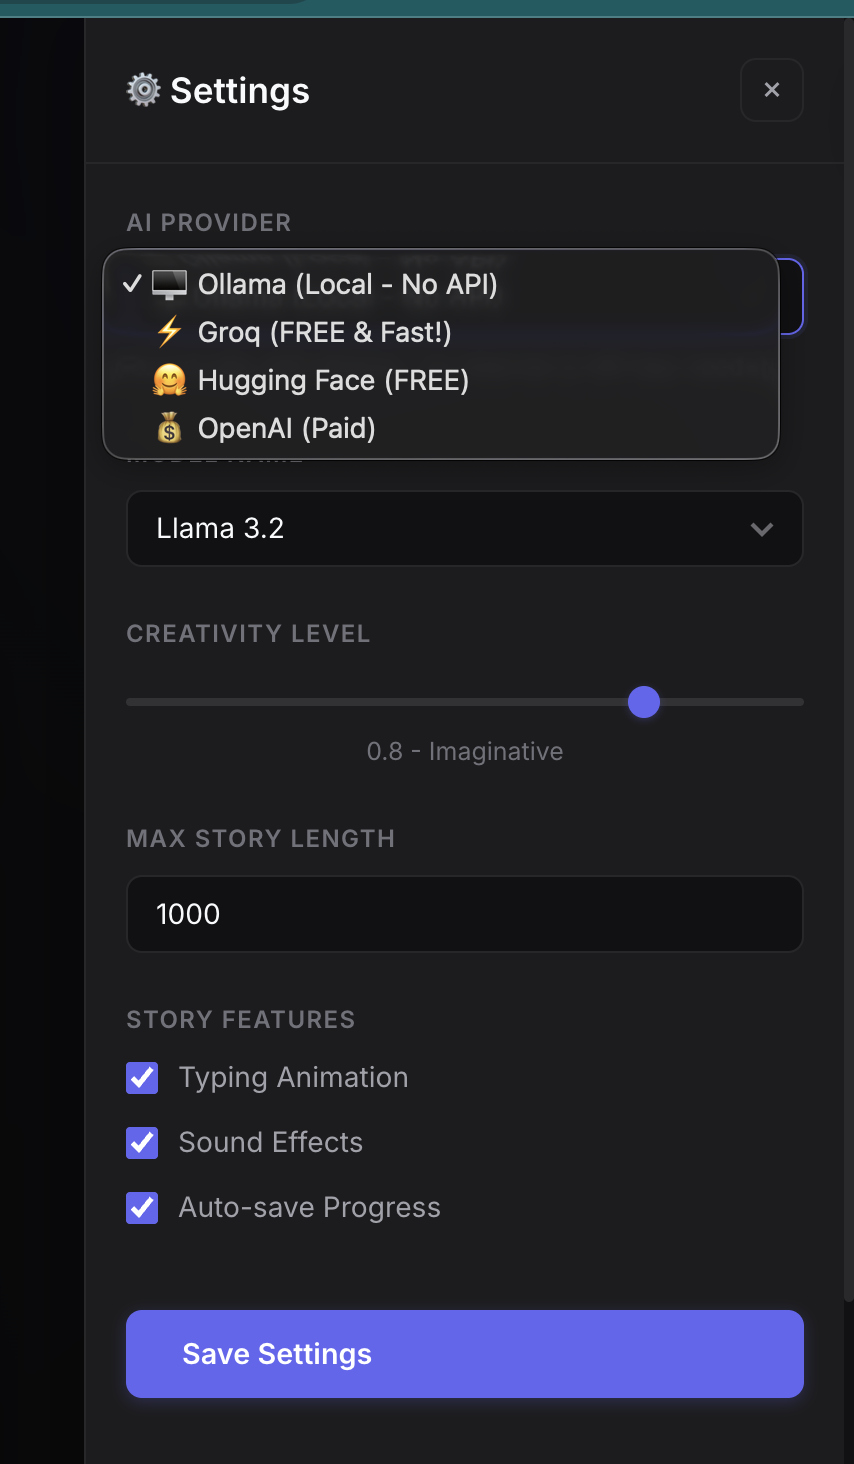
\includegraphics[width=0.55\textwidth]{images/s05_settings.png}
    \caption{Settings panel for provider, model, temperature and feature toggles.}
    \label{fig:ui-settings}
\end{figure}

\subsection{Module 6: Story Flow Manager}

This module implements the five-phase state machine of Section~\ref{sec:phases}. A \texttt{CharacterTracker} records each character's mentions and traits, and a \texttt{PlotThreadTracker} records open plot threads. The consistency checker uses both to flag five kinds of problem: character contradictions, abandoned plot threads, pacing problems, setting inconsistencies and tone shifts.

\subsection{Module 7: Output Formatter}

The formatter cleans the model's output by collapsing extra whitespace and fixing quote and dash characters, splits text at sentence boundaries, wraps dialogue in styled HTML spans, and exports the full story as plain text, Markdown or HTML.

\section{Multimodal Pipelines}

\subsection{Scene Illustration}

For each segment, a short image prompt is built from the most visual sentence. Dialogue in quotation marks and sentences built around thought verbs (\emph{thought, remembered, wondered}) are removed first, because they describe things that cannot be drawn. Each remaining sentence $s$ is scored as
\begin{equation}
\mathrm{score}(s) = 2 \cdot \mathbf{1}_{V}(s) - 2 \cdot \mathbf{1}_{T}(s) + \min\bigl(3,\ |\mathrm{ProperNouns}(s)|\bigr),
\end{equation}
where $\mathbf{1}_V(s)$ is 1 if the sentence contains a visual verb (\emph{stood, loomed, soared, glowed, towered}, and so on) and $\mathbf{1}_T(s)$ is 1 if it contains a thought verb. The best sentence is combined with the genre, the current mood and a fixed style prefix, and the prompt is limited to 200 characters. The pipeline is shown in Figure~\ref{fig:imgpipe}.

\begin{figure}[H]
    \centering
    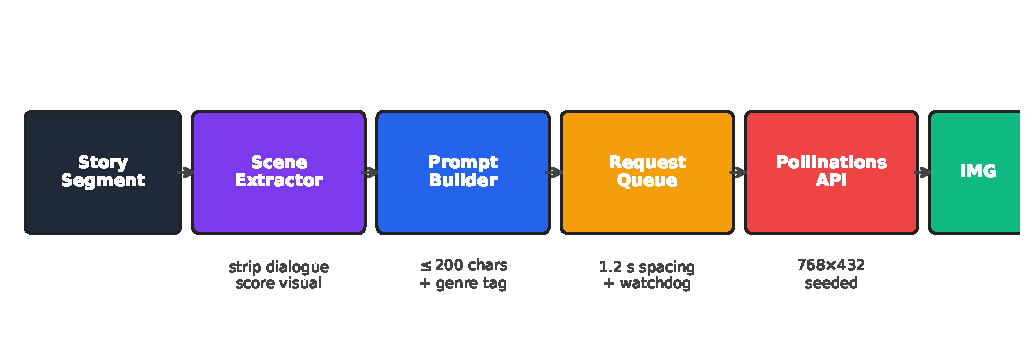
\includegraphics[width=0.95\textwidth]{images/f09_imgpipe.pdf}
    \caption{Per-segment image synthesis pipeline.}
    \label{fig:imgpipe}
\end{figure}

The prompt is sent to Pollinations.ai as a URL:

\begin{lstlisting}
imageUrlFor(segmentText, seed, opts={}) {
    const prompt = this.buildImagePrompt(segmentText, opts);
    const params = new URLSearchParams({
        width: '768', height: '432', nologo: 'true',
        seed: String(seed)
    });
    return `https://image.pollinations.ai/prompt/${encodeURIComponent(prompt)}?${params}`;
}
\end{lstlisting}

Pollinations is served through Cloudflare, which rejects bursts of parallel requests. All image requests therefore pass through a serial queue that sends one request at a time, waits 1.2\,s between requests, and abandons a request after a 35\,s watchdog so that a hung request cannot block the queue. Figure~\ref{fig:ui-loading} shows the loading state while the LLM call and the image request run, and Figure~\ref{fig:ui-story} shows a finished segment with its illustration.

\begin{figure}[H]
    \centering
    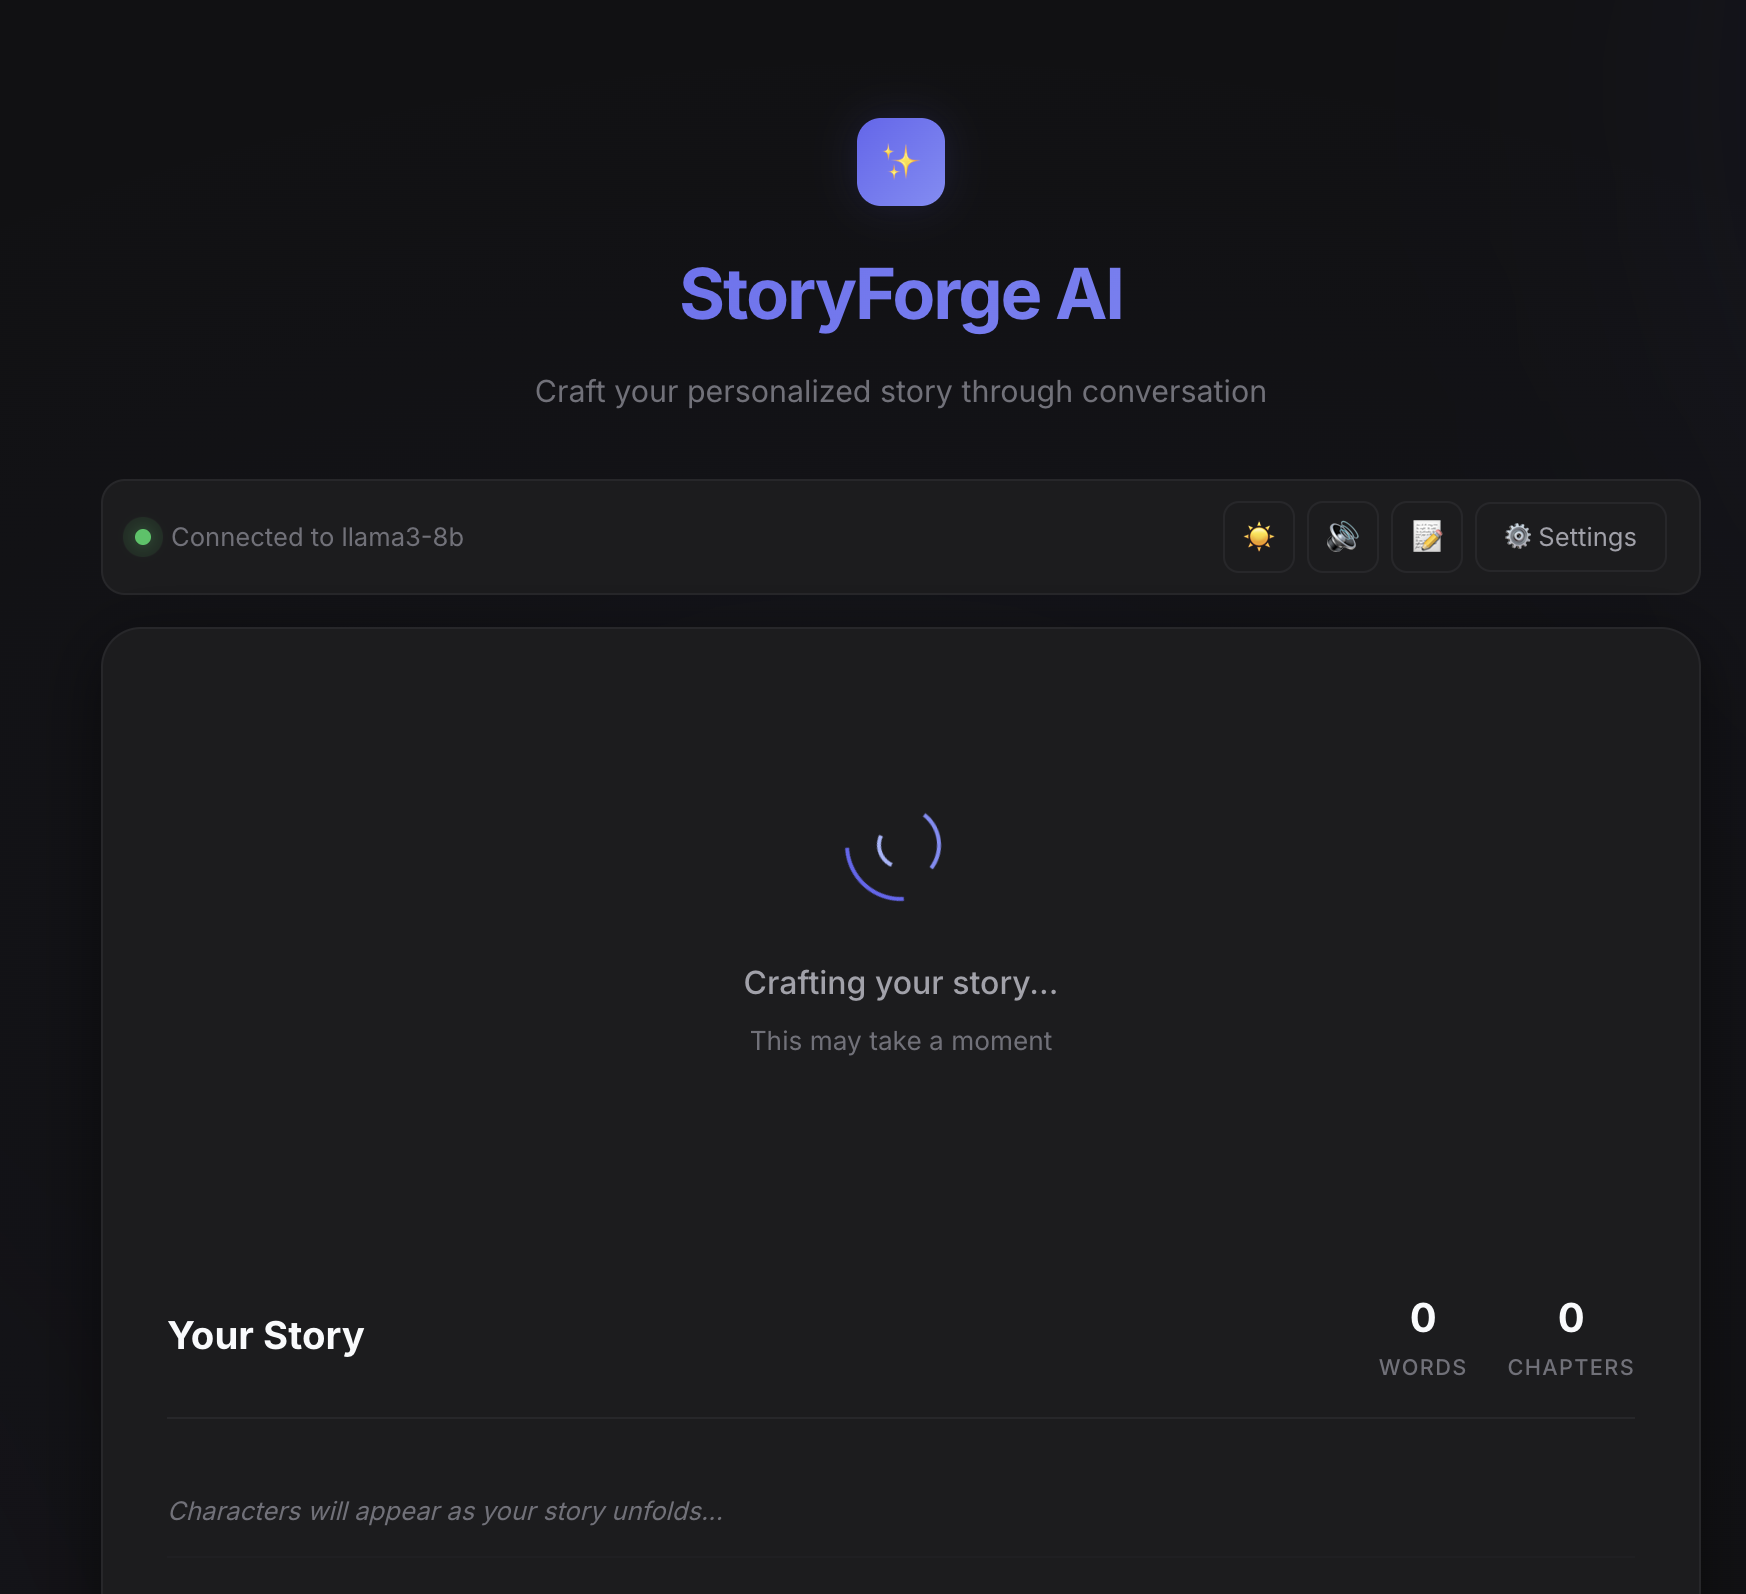
\includegraphics[width=0.85\textwidth]{images/s03_loading.png}
    \caption{Loading state during story and image generation.}
    \label{fig:ui-loading}
\end{figure}

\begin{figure}[H]
    \centering
    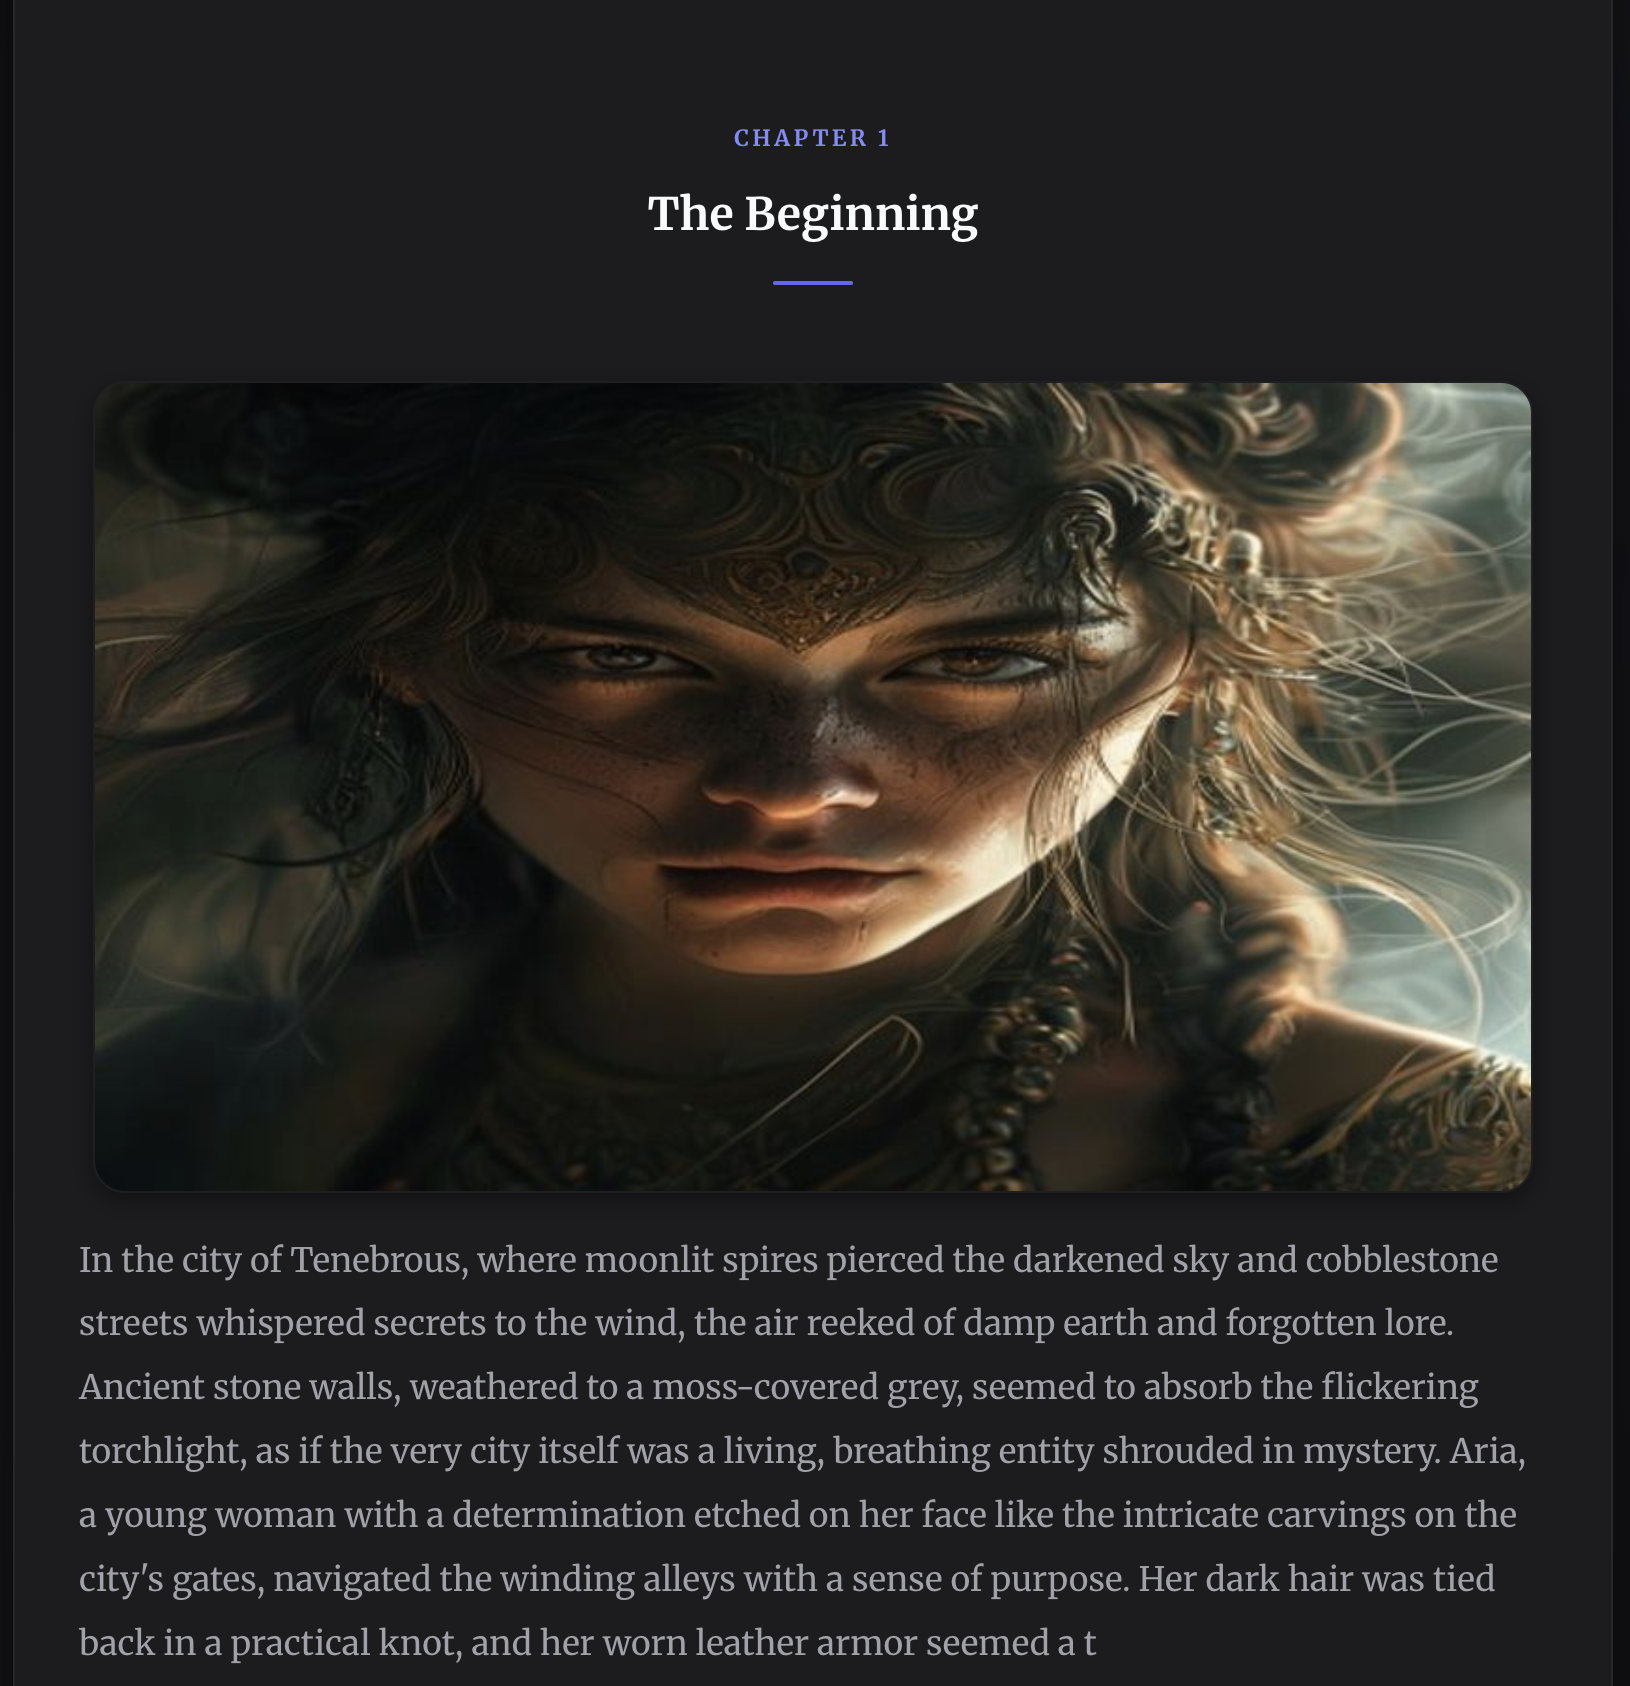
\includegraphics[width=0.65\textwidth]{images/s04_story_image.png}
    \caption{Generated story segment with its scene illustration.}
    \label{fig:ui-story}
\end{figure}

\subsection{Narration and Ambient Music}

The two audio pipelines are shown in Figure~\ref{fig:audio}. Narration uses the browser's \texttt{window.speechSynthesis} interface. One utterance is queued per segment, with pause, resume and stop controls, and the voice is the one provided by the operating system. Ambient music maps each of eight genres to a SoundHelix track, played through \texttt{HTMLAudio} in a loop with a 2.4\,s fade-in and a 0.8\,s fade-out. The \texttt{crossOrigin} attribute is not set, because the CDN does not return CORS headers; setting it caused loading to fail in an early version.

\begin{figure}[H]
    \centering
    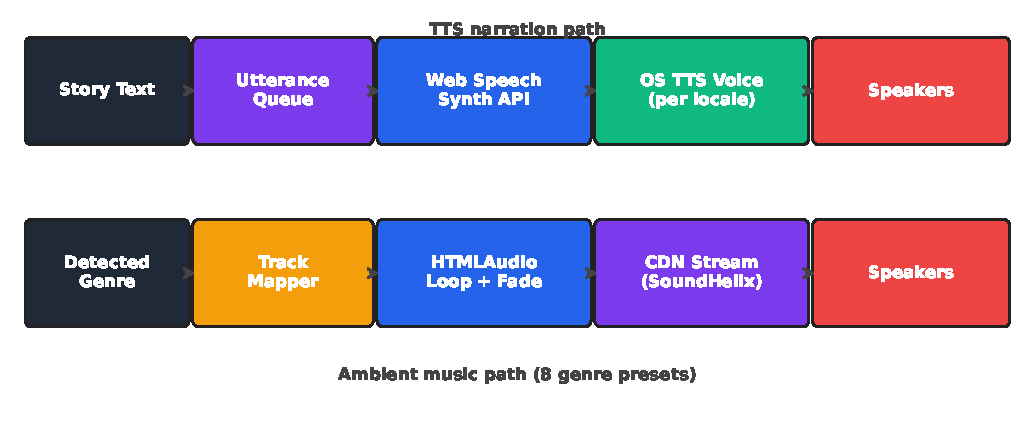
\includegraphics[width=0.95\textwidth]{images/f10_audio.pdf}
    \caption{Narration and ambient-music signal flows.}
    \label{fig:audio}
\end{figure}

\section{Reader Analytics}

\subsection{Story Map}

The Story Map arranges the chapters as a vertical tree using \texttt{d3.tree()}. Each node shows an 80-character preview of its chapter and the user choice that led to it, so the reader can see how the story branched.

\subsection{Character Relationship Graph}

Capitalised words are taken from the segment text and filtered with an extended stop-word list. Only names that appear at least twice are kept. For every pair of kept names, the edge weight is the number of segments in which both appear, and the node radius grows with the number of mentions. The graph is drawn with a D3 force layout (link distance 110, charge $-220$, collision radius 34 pixels). Because the edges are based only on co-appearance, the modal states clearly that the graph shows which characters appear together and not the type of relationship between them.

\section{System Implementation}

\subsection{Project Structure}

The source code is organised as follows and is available as open source~\citep{jha2026repo}:

\begin{lstlisting}
AI-Story-Generator/
|-- main.py                    # FastAPI entry point, REST endpoints
|-- config.py                  # provider, model, temperature
|-- requirements.txt
|-- app/
|   |-- modules/
|   |   |-- user_input.py            # 17 questions, 4 phases
|   |   |-- context_extraction.py    # StoryContext + custom_elements
|   |   |-- knowledge_memory.py      # SQLite + LRU cache
|   |   |-- prompt_engineering.py    # 6 prompt families
|   |   |-- story_generator.py       # BaseLLMClient + 4 providers
|   |   |-- story_flow_manager.py    # 5-phase FSM + trackers
|   |   `-- output_formatter.py      # TXT/MD/HTML export
|   |-- templates/index.html         # single-page shell
|   `-- static/css/style.css, js/app.js
`-- data/storytelling.db
\end{lstlisting}

\subsection{Database Schema}

The SQLite database has five tables:

\begin{lstlisting}
sessions         (session_id PK, user_id, created_at, status)
story_segments   (id PK, session_id FK, order, content, user_choice)
story_context    (session_id PK/FK, context_json, updated_at)
qa_history       (id PK, session_id FK, question_id, q_text, a_text)
user_preferences (user_id PK, preferences_json, updated_at)
\end{lstlisting}

\subsection{REST API}

The server exposes the endpoints listed in Table~\ref{tab:rest}. All request and response bodies are typed with Pydantic~v2.

\begin{table}[H]
\centering
\caption{REST API endpoints.}
\label{tab:rest}
\renewcommand{\arraystretch}{1.2}
\small
\begin{tabular}{|l|c|l|}
\hline
\textbf{Endpoint} & \textbf{Method} & \textbf{Purpose} \\
\hline
\texttt{/}                           & GET    & Web interface \\
\texttt{/api/status}                 & GET    & Check LLM availability \\
\texttt{/api/session/new}            & POST   & Create a new session \\
\texttt{/api/questions/all}          & GET    & All questions, grouped by phase \\
\texttt{/api/question/next}          & GET    & Next question (sequential mode) \\
\texttt{/api/response}               & POST   & Submit an answer \\
\texttt{/api/story/generate}         & POST   & Generate the first segment \\
\texttt{/api/story/continue}         & POST   & Continue from a user choice \\
\texttt{/api/story/full/\{id\}}      & GET    & Full story of a session \\
\texttt{/api/story/download/\{id\}}  & GET    & Export as TXT, MD or HTML \\
\texttt{/api/settings}               & POST   & Switch provider or model \\
\texttt{/api/session/\{id\}/summary} & GET    & Session statistics \\
\texttt{/api/session/\{id\}}         & DELETE & End a session \\
\hline
\end{tabular}
\end{table}

\subsection{Technology Stack}

The software used is listed in Table~\ref{tab:stack}. All components are free, and most are open source.

\begin{table}[H]
\centering
\caption{Technology stack.}
\label{tab:stack}
\renewcommand{\arraystretch}{1.2}
\small
\begin{tabular}{|l|l|l|}
\hline
\textbf{Layer} & \textbf{Technology} & \textbf{Purpose} \\
\hline
Operating system & macOS 14 / Ubuntu 22.04          & Development host \\
Backend language & Python 3.9+                      & Core logic \\
Web framework    & FastAPI with Uvicorn             & REST API and templates \\
Frontend         & HTML5, CSS3, JavaScript          & Single-page interface \\
Visualisation    & D3.js v7                         & Story Map, Character Graph \\
Database         & SQLite3 with aiosqlite           & Sessions, answers, segments \\
HTTP client      & httpx (async)                    & Calls to LLM providers \\
Schemas          & Pydantic v2                      & Request and response types \\
Image service    & Pollinations.ai                  & Text-to-image \\
Speech           & W3C Web Speech Synthesis API     & Narration \\
Ambient audio    & HTMLAudio with SoundHelix        & Genre music \\
LLM providers    & Ollama, Groq, Hugging Face, OpenAI & Story generation \\
\hline
\end{tabular}
\end{table}

\subsection{Hardware Requirements}

Development and evaluation were done on an Apple MacBook Pro with an M2 Pro processor (10-core CPU, 16-core GPU), 16\,GB unified memory, a 1\,TB SSD and a 100\,Mbps broadband link. For running models locally through Ollama, the recommended minimum is an 8-core CPU, 16\,GB RAM and 30\,GB of free disk space for model weights. A GPU with 8\,GB or more of memory speeds up local inference but is not needed when the Groq cloud is used.

\subsection{Implementation Size}

Table~\ref{tab:loc} gives the approximate size of the implementation.

\begin{table}[H]
\centering
\caption{Implementation size in lines of code.}
\label{tab:loc}
\renewcommand{\arraystretch}{1.2}
\begin{tabular}{|l|r|}
\hline
\textbf{Component} & \textbf{Lines of code} \\
\hline
Python backend (7 modules, main, config) & $\approx$ 3,800 \\
Frontend JavaScript                      & $\approx$ 1,700 \\
Frontend CSS                             & $\approx$ 2,200 \\
HTML template                            & $\approx$ 400 \\
Tests and tooling                        & $\approx$ 300 \\
\hline
\textbf{Total}                           & $\approx$ \textbf{8,400} \\
\hline
\end{tabular}
\end{table}

\section{Evaluation Method}
\label{sec:evalmethod}

The system was evaluated in three ways:

\begin{enumerate}
    \item \textbf{Automatic generation.} Fifty stories were generated across six genres and all four question budgets. Latency, token usage and the output of the consistency checker were recorded for every call.
    \item \textbf{User study.} Fifteen participants (8 male, 7 female, aged 22--35, with both technical and non-technical backgrounds) each created two stories, giving 30 stories in total. They rated each story on a five-point Likert scale for coherence, creativity, engagement and consistency, and rated their satisfaction with each feature.
    \item \textbf{Consistency-checker evaluation.} Fifty segments were annotated by hand for the five problem types, and the checker's detection rate and false-positive rate were measured against these annotations.
\end{enumerate}

The following measures were used:

\begin{itemize}
    \item \textbf{Latency}: mean time in seconds for the first segment and for a continuation, measured end to end.
    \item \textbf{Likert score}: mean rating from 1 (poor) to 5 (excellent) for each dimension.
    \item \textbf{Detection rate and false-positive rate} of the consistency checker for each problem type.
    \item \textbf{Precision, recall and $F_1$} for character extraction, where
    \begin{equation}
    P = \frac{TP}{TP+FP}, \qquad R = \frac{TP}{TP+FN}, \qquad F_1 = \frac{2PR}{P+R}.
    \end{equation}
    \item \textbf{Image failure rate}: the share of image requests that failed under parallel load.
\end{itemize}

\section{Ethical Considerations}

Generated stories may contain unsuitable content if the user asks for it or if the model produces it by mistake. The system relies on the safety filters of the underlying providers and uses system prompts that ask for content suitable for a general audience. Participants in the user study took part voluntarily, gave informed consent, and could stop at any time. No personal data beyond the story answers was collected, and results are reported only as averages. Generated images and audio are used only for research and education, in line with the terms of the services used.

\section{Summary}

This chapter described the proposed system from feasibility and planning to implementation. The main ideas are a structured but extensible Q\&A protocol, the \texttt{custom\_elements} channel that carries user-added questions into the prompt, a five-phase story model that keeps the plot on course, a provider-independent LLM layer, and multimodal pipelines that are paced to work reliably with free services. The next chapter presents the results obtained with this system.
